\documentclass[10pt,twocolumn]{article}
\usepackage[utf8]{inputenc}
\usepackage[
  letterpaper,
  top=0.75in, bottom=1in,
  left=0.75in, right=0.75in,
  columnsep=0.25in
]{geometry}
\usepackage{times}
\usepackage{booktabs}
\usepackage{graphicx}
\usepackage{times}
\usepackage[T1]{fontenc}

% ── Core packages ─────────────────────────────────────────────────────────────
\usepackage{multicol}
\usepackage{booktabs}
\usepackage{microtype}
\usepackage{graphicx}
\usepackage{caption}
\usepackage{subcaption}
\usepackage{amsmath}
\usepackage{amssymb}
\usepackage{balance}
\usepackage{hyperref}
\usepackage{enumitem}
\usepackage{xcolor}
\usepackage{titlesec}
\usepackage{abstract}
\usepackage{fancyhdr}
\usepackage{parskip}
\usepackage{array}
\usepackage{tabularx}

% ── Section heading style (ACM uses bold, smaller caps) ──────────────────────
\titleformat{\section}{\normalsize\bfseries\scshape}{}{0em}{}
\titleformat{\subsection}{\normalsize\bfseries}{}{0em}{}
\titleformat{\subsubsection}{\normalsize\itshape}{}{0em}{}
\titlespacing{\section}{0pt}{8pt plus 2pt minus 2pt}{4pt plus 1pt}
\titlespacing{\subsection}{0pt}{6pt plus 2pt minus 1pt}{3pt plus 1pt}

% ── Abstract styling ─────────────────────────────────────────────────────────
\renewenvironment{abstract}{%
  \small\bfseries Abstract ---\normalfont\small\hspace{0.5em}%
}{}

% ── Caption styling ──────────────────────────────────────────────────────────
\captionsetup{font=small, labelfont=bf, skip=4pt}

% ── No paragraph indentation, small paragraph skip ───────────────────────────
\setlength{\parindent}{9pt}
\setlength{\parskip}{2pt}

% ── Header / footer ──────────────────────────────────────────────────────────
\pagestyle{fancy}
\fancyhf{}
\fancyhead[C]{\small\textit{CS 6120 Final Paper --- Northeastern University, Seattle, 2025}}
\fancyfoot[C]{\thepage}
\renewcommand{\headrulewidth}{0.4pt}

% ── Hyperref config ───────────────────────────────────────────────────────────
\hypersetup{
  colorlinks=true, linkcolor=black, citecolor=black, urlcolor=blue,
  pdftitle={Iterative Decay on Human Style through LLM Paraphrasing},
  pdfauthor={Jae Hun Cho, Catherine Nguyen}
  }

\title{\textbf{Iterative Decay on Human Style through LLM Paraphrasing}}

\author{Jae Hun Cho\\
  Northeastern University, Seattle, WA, USA\\
  \texttt{cho.jae@northeastern.edu}
  \and
  Catherine Nguyen\\
  Northeastern University, Seattle, WA, USA\\
  \texttt{nguyen.cathe@northeastern.edu}
}

\date{}


\begin{document}
\maketitle

% \begin{abstract}
% We investigate whether LLM-based paraphrasers preserve or attenuate syntactic complexity. If the paraphrasing process systematically strip away syntactic complexity, does it create more generalized and accessible information at the cost of stylistic structure and the original author's semantic intent?
% \end{abstract}

\section{Abstract}

Whether they are academics, literary authors, or posters on internet forums, human writers craft sentences with unique cadences and syntactic structure. Linguistic syntax can vary from simple sentences to complex nested clauses with long-range dependencies. LLMs are often used to summarize and improve the readability of complex literature such as articles or science publications, but \textbf{do LLMs preserve the original sentence structure, or does it gradually erode syntactic diversity towards a median complexity.}

This project will investigate whether LLM paraphrasers exhibit an inherent simplification bias that progressively flattens syntactic structures across iterative transformations (T0→T1→T2→T3). Through tracking syntactic decay, we can see if the simplification of stylistic structure alters the overall semantics of the text. In addition, we also see if different LLM paraphrasers approach similar levels of syntactic complexity, or if other models preserve the sophistication better than others.

This research will provide insight into: (1) \textbf{Academic Integrity}: detecting AI-laundered writing; (2) \textbf{Accessibility vs. Quality}: understanding whether simplification aids comprehension or smoothens over nuance; (3) \textbf{Model Fingerprinting}: identifying LLMs based on their levels of syntactic flattening.

\section{Background}

Asthana et al.\cite{asthana2024} introduces targeted domain-specific concept simplification to improve human reading comprehension on these difficult-to-navigate concepts. They created a dataset of 22k definitions from 13 academic domains with annotated difficult concepts, and evaluated LLMs using three approaches: dictionary definitions, simplification, and contextual explanation. Human evaluations showed preference for contextual explanations over lexical simplifications or substitutions.

Dong et al.\cite{dong2017} explores how question answering (QA) systems struggle to express the same information in many different ways in natural language. They utilize paraphrase generating to capture the knowledge required to answer a question and present a general framework  which learns suitable paraphrases for various QA tasks. They found that the framework consistently improved QA performance from learning task-specific paraphrases.

Feng et al.\cite{feng2010} compares various features for automatic readability assessment of primary school reading materials. The researchers extracted and evaluated discourse features (entity-density, lexical chains), language modeling features, POS-based features, syntactic features, and shallow features using classification models. Language models trained on in-domain data had the highest predictive power, and their judicious feature combination achieved 74\% classification accuracy, significantly improving over the 63\% state-of-the-art.

Xu et al.\cite{xu2015} argues that Simple Wikipedia, the dominant simplification dataset, is inadequate due to alignment errors and incomplete simplifications. The authors introduced the Newsela corpus, professionally simplified news articles across multiple grade levels and conducted comparative analyses. Manual examination revealed that Simple Wikipedia sentence pairs are not true simplifications, whereas Newsela provides more consistent, higher-quality simplifications.

Zheng et al.\cite{zheng2018} addresses run-on sentence correction. They developed two models—a CRF model (roCRF) and a Seq2Seq attention model (roS2S)—and experimented with artificially generated training data from clean newswire text. The roS2S model achieved strong performance (F0.5 = 0.86 on clean data), and models trained on artificial data performed nearly as well on real run-ons, suggesting artificial training data is viable for low-coverage error types.

\section{Project Plan and Milestones}
\vspace{-5pt}

\begin{table}[h]
\centering
\small
\begin{tabular}{@{}clp{3.8cm}@{}}
\toprule
\textbf{Wk} & \textbf{Phase} & \textbf{Deliverable} \\
\midrule
3-5 & Data \& Complexity Profiling & Extract syntactic features from T0; stratify sentences by complexity \\
6-9 & Baseline \& Erosion Tracking & Define a baseline complexity; Measure syntactic features across T1-T3 iterations \\
10-12 & Model Comparison & Compare syntactic conservatism across models by structural fidelity \\
13-14 & Analysis & Build interactive dashboard with analysis of syntactic complexity
decay visualizations \\
\bottomrule
\end{tabular}
\end{table}

\section{Research Questions}

We investigate three important pillars of LLM paraphrasing:

\textbf{RQ1 (Style vs.\ Content Decay):} Which linguistic ``planks'' are replaced
first? We compare the decay rate of stylistic features (e.g., POS-tag
frequencies, sentence length variance) against semantic content (e.g.,
BERTScore F1) across T1, T2, and T3.

\textbf{RQ2 (Point of No Return):} At what iteration does a text effectively
``lose'' its original identity? Does authorship attribution performance
collapse sharply at T1 or gradually across the chain?

\textbf{RQ3 (Paraphraser Fingerprints):} Do different paraphrasers (ChatGPT,
PaLM2, Pegasus, Dipper) leave distinct signatures in the transformed text?
Can we identify which paraphraser was used based on the residual style?

\section{Dataset and Corpus}

\subsection{The Ship of Theseus Corpus}
We will use the Ship of Theseus \cite{tripto2024} which contains iterative paraphrase chains across multiple source datasets. The corpus maps text change through four iterations:

\begin{itemize}[leftmargin=*,topsep=2pt,itemsep=1pt]
  \item \textbf{T0:} Original human-authored text
  \item \textbf{T1:} First paraphrase iteration
  \item \textbf{T2:} Second paraphrase (of T1)
  \item \textbf{T3:} Third paraphrase (of T2)
\end{itemize}

\noindent Each source document has seven paraphrasers, and seven sources (Human or LLM writers).

\subsection{Source Datasets}
We work with seven source datasets spanning diverse text domains:

\begin{center}
\small
\begin{tabular}{lll}
\toprule
\textbf{Dataset} & \textbf{Domain} & \textbf{Style} \\
\midrule
sci\_gen  & Scientific    & Formal, technical \\
wp        & Creative fiction & Narrative, diverse \\
xsum      & News summaries & Journalistic \\
eli5      & Explanatory QA & Informal, varied \\
cmv       & Debate/persuasion & Argumentative \\
tldr      & Summarization & Compressed \\
yelp      & Reviews       & Colloquial \\
\bottomrule
\end{tabular}
\end{center}

\noindent This diversity is intentional: we expect paraphrase decay to manifest
differently across domains. Formal scientific text with domain-specific
vocabulary may resist lexical simplification differently than colloquial
review text.

\subsection{Paraphrasers}
Four paraphraser groups are represented in the corpus:

\begin{itemize}[leftmargin=*,topsep=2pt,itemsep=1pt]
  \item \textbf{ChatGPT}: Instruction-tuned large LLM
  \item \textbf{PaLM2}: Large language model
  \item \textbf{Pegasus(slight/full)}: Seq2seq summarization model
  \item \textbf{Dipper(low/high)}: Discourse paraphraser
\end{itemize}

\noindent Paraphraser variants (e.g., \texttt{dipper(high)}, \texttt{pegasus(slight)}) are grouped into the above mentioned family for cross-paraphraser analysis. The version\_name column in the data set denotes the iteration of the text: \texttt{chatgpt\_chatgpt\_chatgpt} indicates that it is the third ChatGPT iteration (T3).

\subsection{Dataset Statistics}

Table~\ref{tab:corpus_stats} summarizes the loaded corpus. Document counts
at T0 reflect unique source texts; T1--T3 counts are higher because each
T0 document has chains for multiple paraphrasers.

\begin{center}
\small
\begin{tabular}{lrrr}
\toprule
\textbf{Dataset} & \textbf{T0 docs} & \textbf{Total rows} \\
\midrule
sci\_gen  & 2797  & 60,166 \\
wp        & 2768  & 58,417 \\
xsum      & 3227  & 70,388 \\
eli5      & 3160  & 69,270 \\
cmv       & 1626  & 35,405 \\
tldr      & 2444  & 53,519 \\
yelp      & 3320  & 72,847 \\
\midrule
\textbf{Total} & \textbf{19,342} & \textbf{420,012} \\
\bottomrule
\end{tabular}
\captionof{table}{Corpus statistics by dataset. Each T0 document generates
up to 7 paraphraser chains across T1--T3.}
\label{tab:corpus_stats}
\end{center}

\section{Methodology}

\subsection{Data Pipeline}
Our pipeline follows a four-stage process implemented in \texttt{src/data/}:

\textbf{Stage 1 -- Loading (\texttt{load\_data.py}):} Raw CSVs are loaded
with validation of expected columns (\texttt{source}, \texttt{key},
\texttt{text}, \texttt{version\_name}). Three derived columns are added:
\texttt{stage} (T0--T3, mapped from underscore count in version\_name),
\texttt{paraphraser} (base model name), and \texttt{family} (model family
grouping).

\textbf{Stage 2 -- Preprocessing (\texttt{preprocess.py}):} Text is
normalized by lowercasing, removing non-alphanumeric characters, and
stripping whitespace. Stopword removal produces a \texttt{no\_stop\_text}
variant alongside \texttt{cleaned\_text}. Text statistics (word count,
unique word count) are computed per row.

\textbf{Stage 3 -- Chain Building (\texttt{split\_data.py}):} Long-format
data is pivoted into wide-format chains. Each row in the output represents
one complete T0$\rightarrow$T3 chain for a (document, source, paraphraser)
triple, with columns \texttt{T0\_text}, \texttt{T1\_text}, \texttt{T2\_text},
\texttt{T3\_text}. T0 is deduplicated and joined onto each paraphraser chain.

\textbf{Stage 4 -- Similarity Scoring:} BLEU-2 and ROUGE-1/L are computed
via batched scoring (\texttt{src/similarity/bleu\_rouge.py}); BERTScore F1
is computed on GPU using the bert-score library
(\texttt{src/similarity/bertscore.py}). All scoring treats T0\_text as
the reference and T1/T2/T3 as hypotheses.

\subsection{Similarity Metrics}
We use three complementary metrics to capture different aspects of similarity:

\textbf{BLEU-2} measures bigram overlap between hypothesis and reference.
It is used exclusively as a \emph{lexical change} metric, not as a semantic
measure --- consistent with the project specification's explicit warning
against using BLEU as a proxy for meaning preservation.

\textbf{ROUGE-1/L} measures unigram recall and longest common subsequence.
ROUGE-L is particularly informative as it captures ordering information,
making it sensitive to syntactic restructuring that BLEU might miss.

\textbf{BERTScore F1} uses contextual embeddings from a pretrained language
model to compute token-level similarity, making it robust to surface-form
variation. A high BERTScore despite low BLEU/ROUGE indicates semantic
preservation without lexical preservation.

\textbf{SBERT Cosine Similarity} encodes each text into a single
sentence-level embedding using Sentence-BERT (\texttt{all-MiniLM-L6-v2})
and computes cosine similarity between the T0 reference and each
paraphrased stage. Unlike BERTScore, which operates at the token level,
SBERT captures holistic sentence-level semantic similarity in a shared
embedding space.

\subsection{Stylometric Feature Extraction}
To address RQ1, we extract six stylometric features from each text using
spaCy (\texttt{en\_core\_web\_sm}):

\begin{itemize}[leftmargin=*,topsep=2pt,itemsep=1pt]
  \item \textbf{Sentence length} (mean and variance): captures syntactic complexity at the sentence level.
  \item \textbf{Type-Token Ratio (TTR)}: ratio of unique words to total words, measuring lexical diversity.
  \item \textbf{Punctuation ratio}: punctuation characters divided by total characters.
  \item \textbf{POS-tag distribution}: normalized frequency of each Universal POS tag.
  \item \textbf{Dependency depth} (mean and max): depth of the dependency parse tree, measuring syntactic nesting.
\end{itemize}

\noindent We compute Jensen-Shannon divergence between POS distributions at each
stage to quantify how far the grammatical structure drifts from the T0
original.

\subsection{Authorship Attribution}
To address RQ2, we train a Logistic Regression classifier on balanced
T0 data (50\% Human, 50\% AI-generated) using TF-IDF features. The model
is trained exclusively on T0 texts and evaluated on T0 (held-out), T1,
T2, and T3. By observing how classification accuracy degrades across
iterations, we identify the ``point of no return'' where the original
authorship signal is lost. We use all seven datasets (3,500 samples total)
with balanced class sampling to avoid majority-class bias.

\subsection{Paraphraser Fingerprinting}
To address RQ3, we train a Random Forest classifier on T1 data to identify
which paraphraser family (ChatGPT, Dipper, Pegasus, PaLM) produced the
text. Features combine TF-IDF unigrams with stylometric features. Feature
importance analysis reveals which linguistic dimensions are most diagnostic
for distinguishing paraphrasers.

\subsection{Implementation Notes}
BLEU and ROUGE are CPU-bound, but BERTScore was
computed on GPU (NVIDIA T4 via Google Colab) with batch size 64.
Tokenization for BLEU used NLTK's \texttt{punkt} tokenizer with smoothing
method 1. Stylometric analysis used 500 sampled chains per dataset across
three focus datasets (wp, xsum, yelp). Identity forensics experiments used
all seven datasets with 500 samples each.

\section{Results}

\subsection{Corpus Characterization}

\begin{figure}[h]
  \centering
  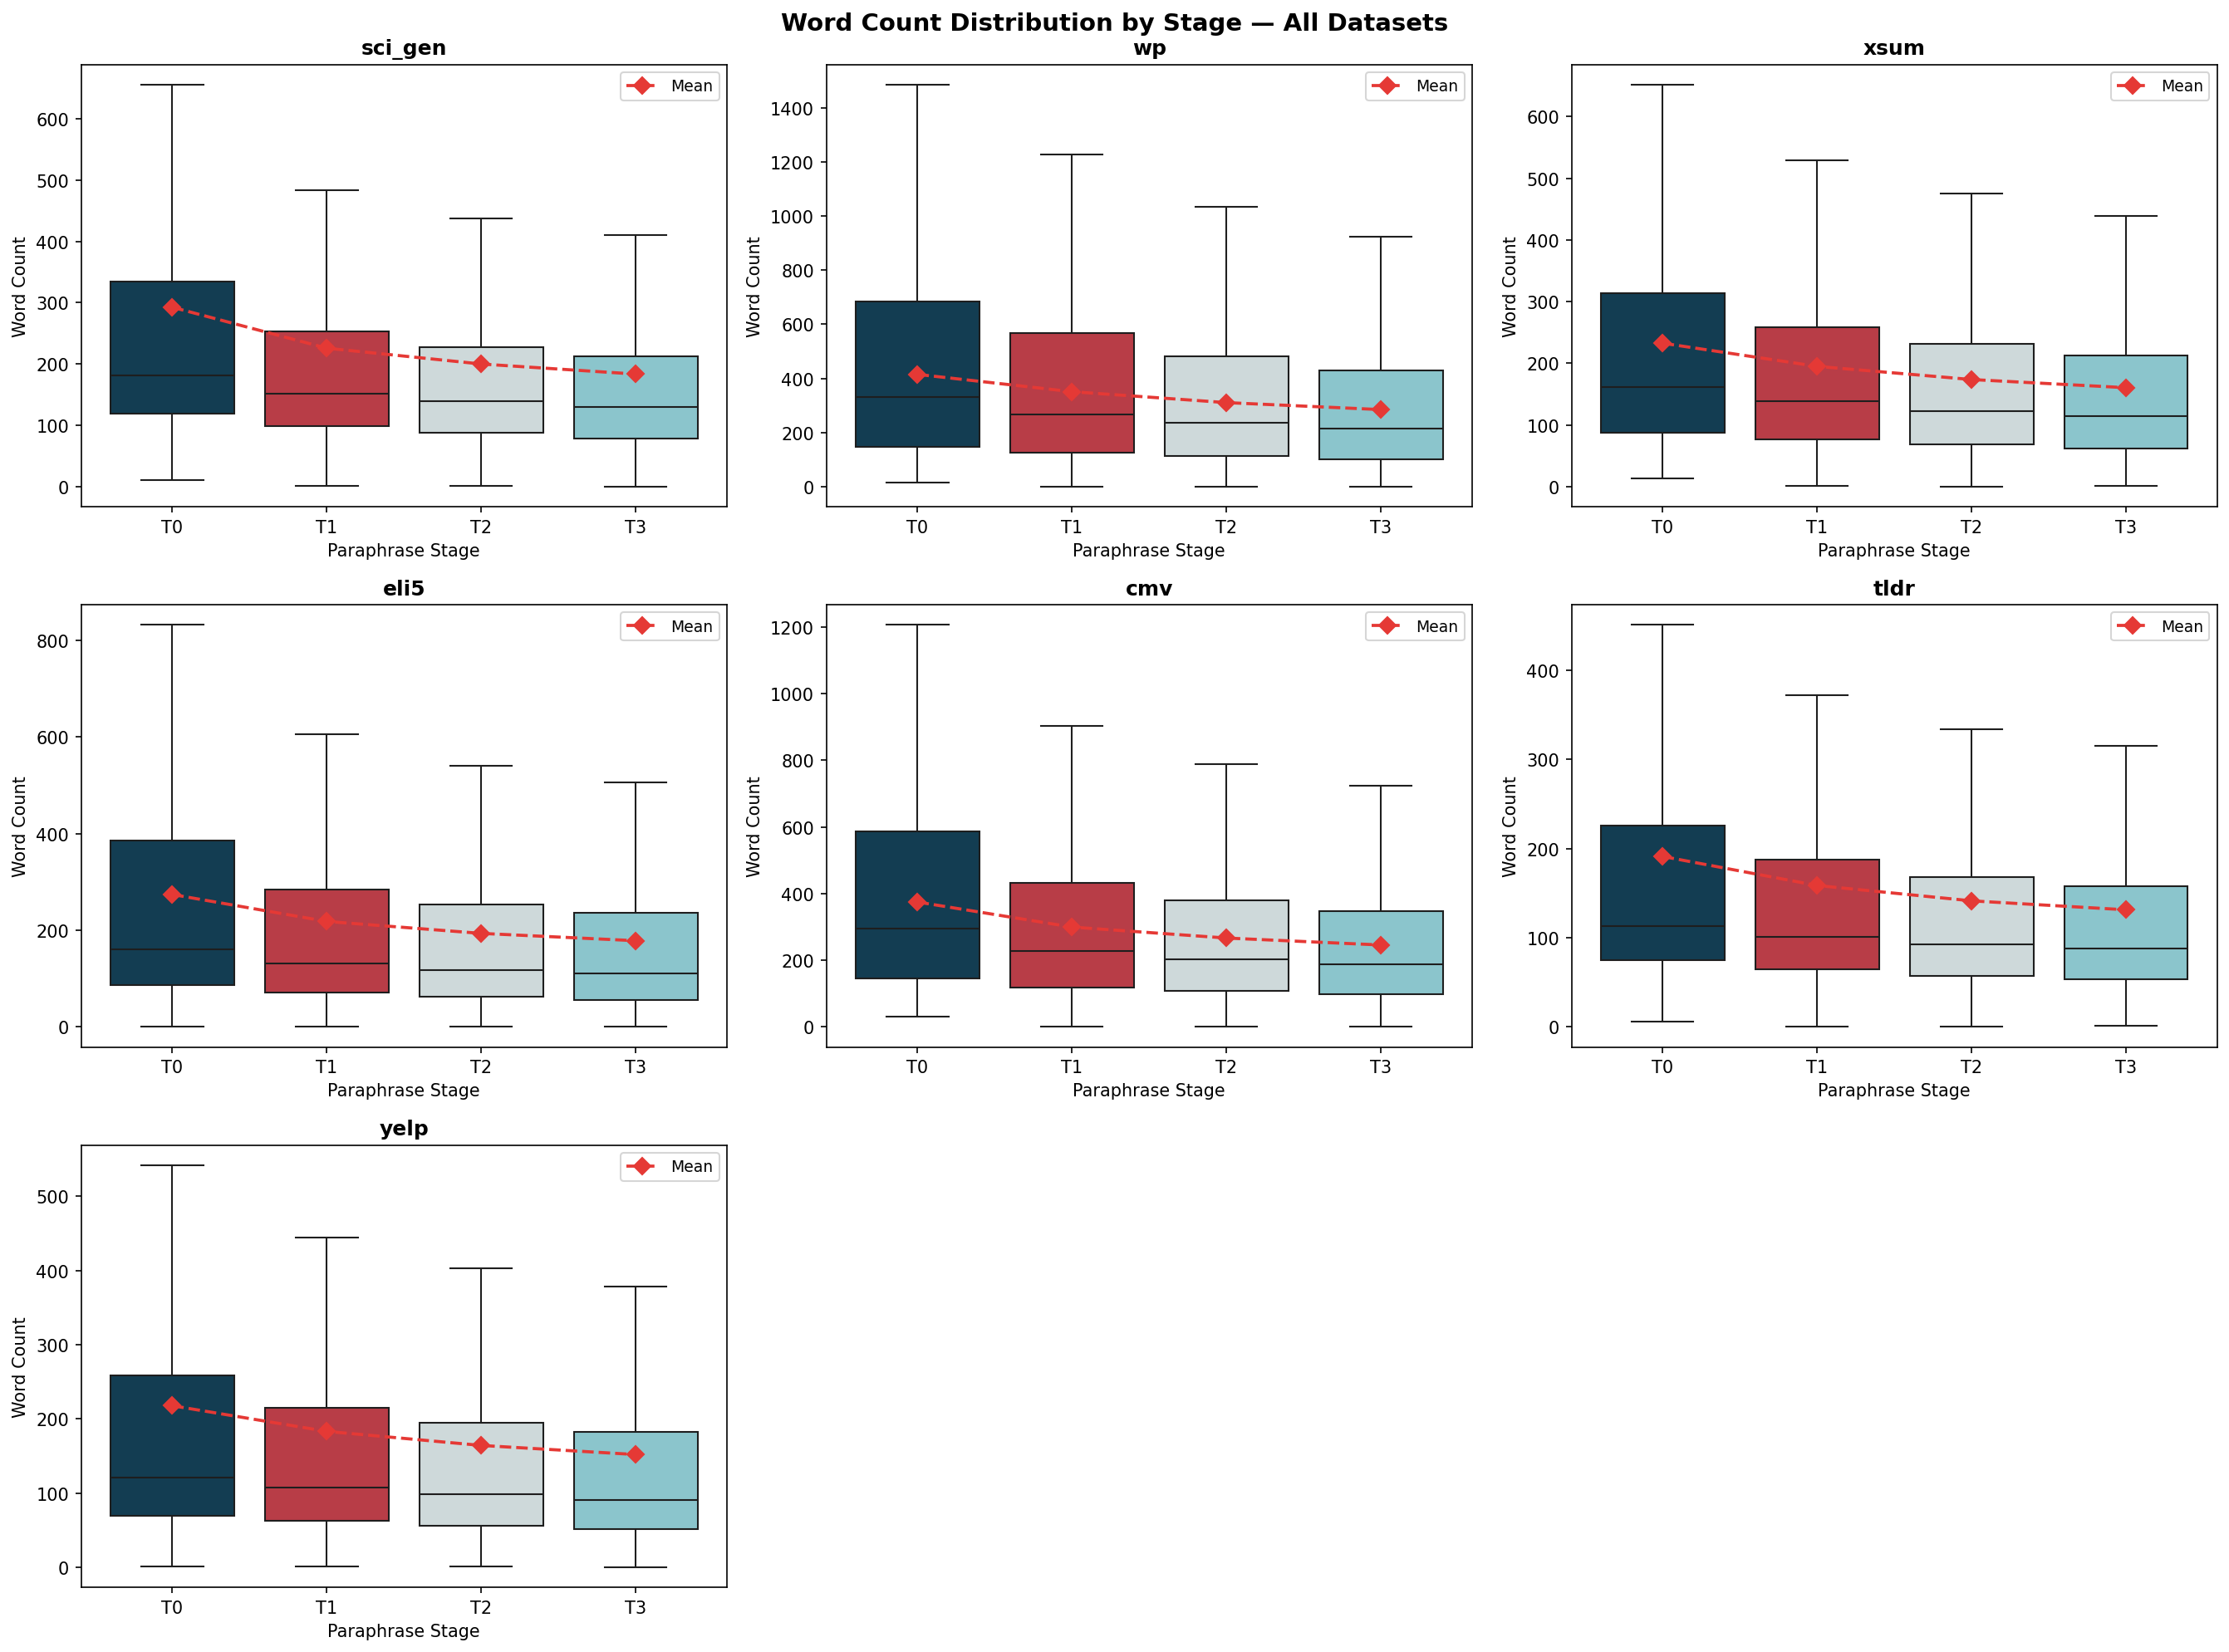
\includegraphics[width=\linewidth]{fig2_word_count_by_stage.png}
  \caption{Word count decay across all seven data sets.}
\end{figure}

\textbf{Word count decay (See Fig. 1)}
shows box plots of word count distribution by stage across all seven datasets.
Mean word count decreases monotonically from T0 to T3 in every dataset.
This finding holds universally: \emph{LLM paraphrasers systematically
shorten text, not merely rephrase it}.

\textbf{Vocabulary reduction.} Comparing all-word counts to content-word
counts (after stopword removal) across stages reveals that both decline in
near-parallel, with content and function words reduced proportionally.

\subsection{Baseline Similarity Analysis}

\textbf{Lexical metrics collapse rapidly (See Fig. 3)} Table~\ref{tab:similarity_means}
presents mean similarity scores across all datasets and paraphrasers. BLEU-2
scores drop sharply from T0 (1.0, reference) to T1, and continue declining
through T3. Across datasets, BLEU-2 at T3 ranges from 0.19 to 0.42, with
the \texttt{wp} creative fiction corpus showing the steepest decline.
ROUGE-1 and ROUGE-L follow similar trajectories but decay less sharply,
consistent with their recall-oriented design that rewards any shared n-gram.

\begin{figure}[h]
  \centering
  
\includegraphics[width=\linewidth]{fig1_lexical_vs_semantic_decay.png}
  \caption{BLEU/ROUGE scores drop drastically after first iteration. However, BERTScore remains relatively stable.}
\end{figure}

\textbf{Semantic similarity is preserved.} BERTScore F1 exhibits a
markedly different decay profile. While BLEU-2 drops below 0.5 by T2 in
most datasets, BERTScore F1 remains above 0.5 through T3 across all
datasets. This divergence is the central quantitative finding of this
update: \emph{lexical planks are replaced before the semantic hull is
compromised}.

\textbf{SBERT confirms semantic preservation at the sentence level.}
SBERT cosine similarity declines from 1.0 (T0) to 0.79 (T1), 0.75 (T2),
and 0.73 (T3). This decay rate is steeper than BERTScore (which remains at
0.81 at T3) but far slower than lexical metrics. The difference between
BERTScore and SBERT is informative: BERTScore's token-level matching is
more forgiving of paraphrasing (it aligns individual tokens), while SBERT's
holistic sentence embedding is more sensitive to structural reorganization.
Per-dataset SBERT scores range from 0.71 (sci\_gen, yelp at T3) to 0.75
(xsum at T3), confirming that semantic preservation holds across all domains.

\begin{center}
\small
\begin{tabular}{lrrrr}
\toprule
\textbf{Metric} & \textbf{T0} & \textbf{T1} & \textbf{T2} & \textbf{T3} \\
\midrule
BLEU-2       & 1.00 & 0.54 & 0.38 & 0.28 \\
ROUGE-1      & 1.00 & 0.67 & 0.54 & 0.46 \\
ROUGE-L      & 1.00 & 0.61 & 0.48 & 0.41 \\
BERTScore F1 & 1.00 & 0.91 & 0.86 & 0.81 \\
SBERT Cosine & 1.00 & 0.79 & 0.75 & 0.73 \\
\bottomrule
\end{tabular}
\captionof{table}{Mean similarity scores (vs.\ T0) across all datasets
combined. Values at T0 = 1.0 by definition (reference against itself).
BERTScore decays approximately 3$\times$ slower than BLEU-2. SBERT cosine
similarity falls between lexical and token-level semantic metrics.}
\label{tab:similarity_means}
\end{center}

\begin{figure}[h]
  \centering
  
\includegraphics[width=\linewidth]{fig1_decay_by_family.png}
  \caption{Paraphraser Families relatively follow the same trend seen previously. Pegasus Family is most conservative in lexical change; conversely, Dipper Family is most aggressive.}
\end{figure}

\textbf{Paraphraser family differences (See Fig. 4)} shows decay curves
stratified by paraphraser family. Pegasus exhibits the most conservative
behavior, maintaining the highest BLEU-2 and ROUGE-L scores at every
iteration which is consistent with its design as a summarization model that
prioritizes concise content. Dipper shows the most aggressive lexical
replacement, with BLEU-2 approaching 0.25 at T3. ChatGPT and PaLM2 fall
between these extremes, with broadly similar profiles. Notably, all four
families show comparable BERTScore F1 profiles, suggesting that semantic
content preservation is a property of the paraphrase task itself rather
than a distinguishing feature of individual models.

%% ════════════════════════════════════════════════════════════════════════════
%% PHASE 2 RESULTS
%% ════════════════════════════════════════════════════════════════════════════

\subsection{Stylometric Profiling (RQ1)}

To move beyond surface-level lexical metrics, we extract syntactic and
stylistic features from each stage using spaCy. Table~\ref{tab:stylometry}
summarizes mean feature values across all sampled texts.

\begin{center}
\small
\begin{tabular}{lrrrr}
\toprule
\textbf{Feature} & \textbf{T0} & \textbf{T1} & \textbf{T2} & \textbf{T3} \\
\midrule
Sent.\ length (mean) & 16.85 & 17.16 & 16.93 & 16.60 \\
Sent.\ length (var)  & 92.64 & 101.94 & 91.03 & 94.99 \\
TTR                   & 0.632 & 0.631 & 0.644 & 0.654 \\
Punct.\ ratio         & 0.033 & 0.031 & 0.031 & 0.031 \\
Dep.\ depth (mean)    & 2.622 & 2.580 & 2.547 & 2.518 \\
Dep.\ depth (max)     & 8.679 & 8.331 & 8.247 & 7.967 \\
\bottomrule
\end{tabular}
\captionof{table}{Stylometric features by stage, averaged across wp, xsum,
and yelp datasets (500 samples each). Dependency depth decreases
monotonically; TTR increases.}
\label{tab:stylometry}
\end{center}

\textbf{Syntactic simplification is consistent.} Mean dependency depth
decreases from 2.622 (T0) to 2.518 (T3), a 3.9\% reduction, while maximum
dependency depth drops from 8.68 to 7.97 ($-$8.2\%). This confirms that
paraphrasers systematically flatten nested syntactic structures across
iterations.

\textbf{Lexical diversity increases.} Counterintuitively, Type-Token Ratio
rises from 0.632 to 0.654 (+3.4\%). Because total word count also decreases
(Section 7.1), this suggests paraphrasers compress text by removing
\emph{repetitive} tokens while retaining diverse vocabulary.

\begin{figure}[h]
  \centering
  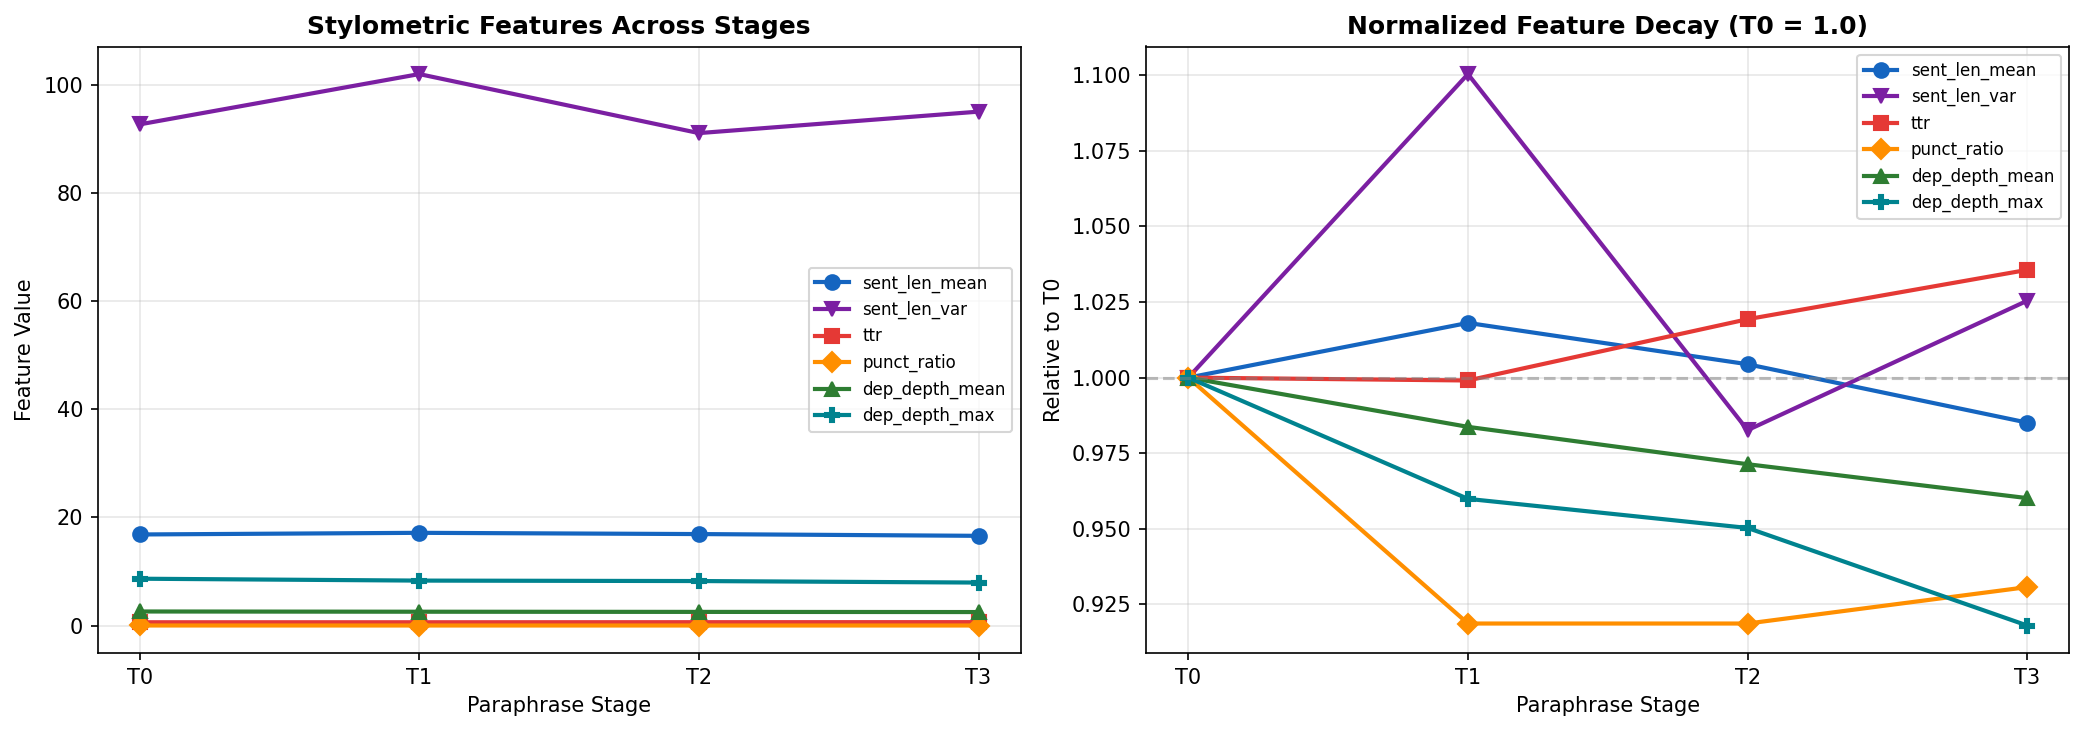
\includegraphics[width=\linewidth]{fig1_feature_decay_curves.png}
  \caption{Normalized stylometric feature values across T0--T3. Dependency
  depth and punctuation ratio decline monotonically; TTR increases.}
\end{figure}

\textbf{POS distributions drift measurably.} While content-word categories
(NOUN, VERB) remain relatively stable, function-word categories (PUNCT,
CCONJ, DET) show visible shifts. Jensen-Shannon divergence between each
stage's POS distribution and the T0 baseline increases monotonically,
confirming progressive grammatical drift from the original.

\begin{figure}[h]
  \centering
  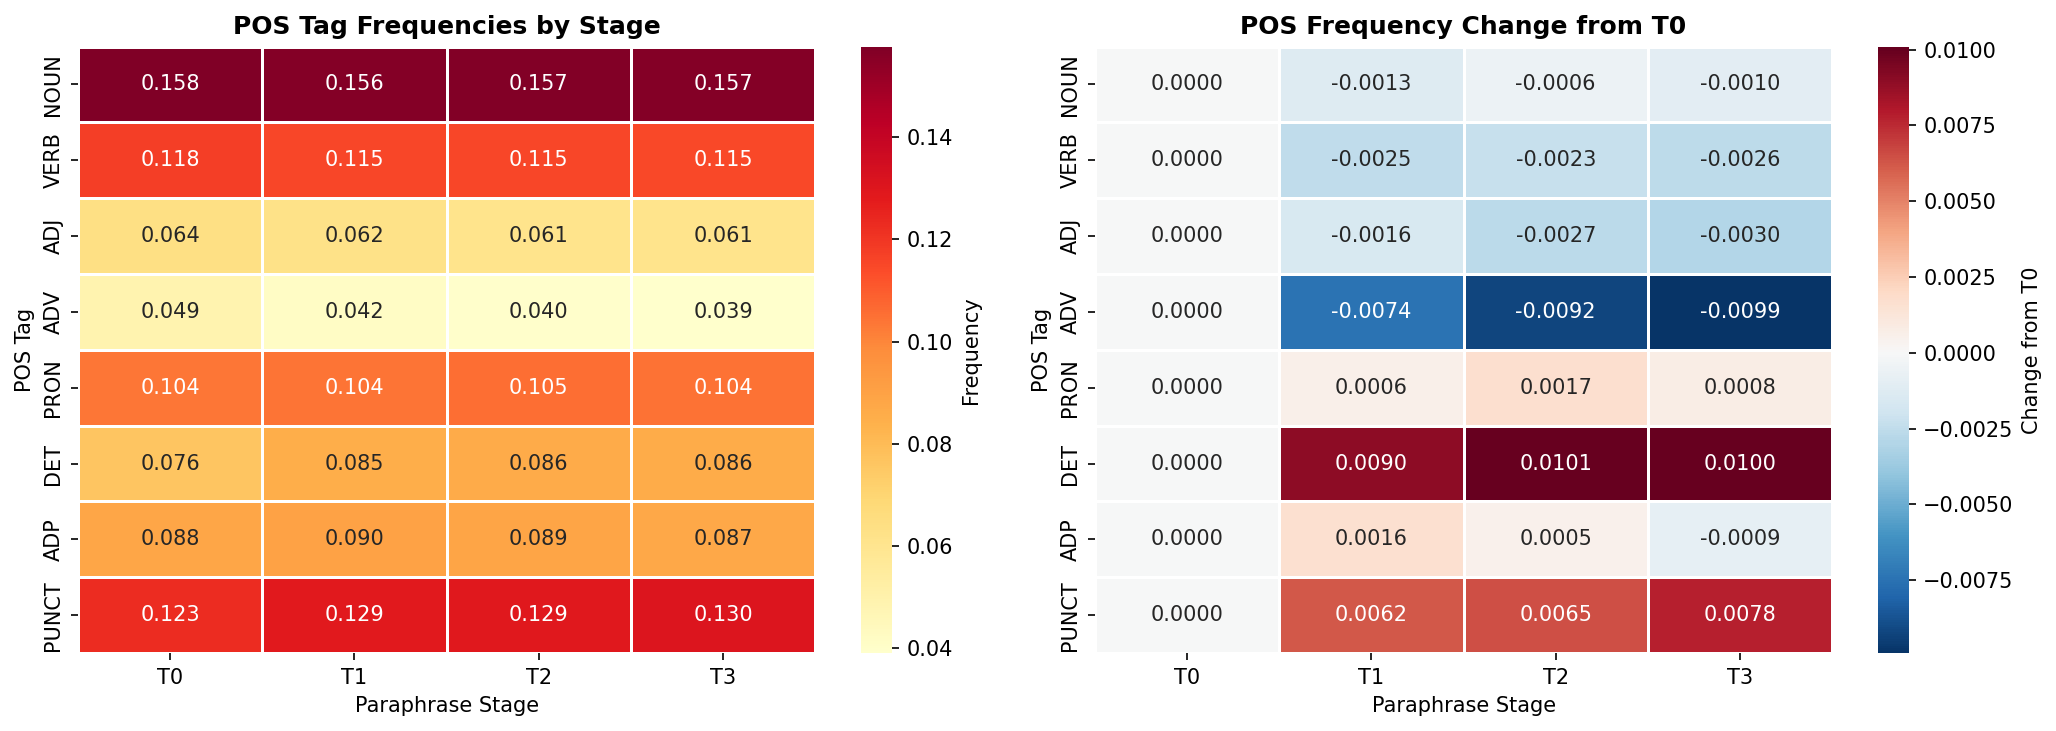
\includegraphics[width=\linewidth]{fig2_pos_heatmap.png}
  \caption{POS tag frequencies by stage (left) and frequency change from T0
  (right). Content-word tags (NOUN, VERB) remain stable across iterations,
  while function-word tags (DET, PUNCT) show consistent directional shifts.
  ADV frequency decreases monotonically ($-$0.0099 by T3); DET and PUNCT
  increase, suggesting paraphrasers insert determiners and punctuation
  while compressing adverbial modifiers.}
  \label{fig:pos_heatmap}
\end{figure}

\subsection{Identity Trajectory}

We project all texts into a shared embedding space using TF-IDF followed by
PCA(50)$\rightarrow$t-SNE(2). The projection shows substantial overlap
between stages, with silhouette scores near zero ($-$0.014 in t-SNE space),
confirming that paraphrased texts do not form separable clusters by
iteration. This supports the metaphor of gradual plank replacement:
each iteration shifts the text incrementally rather than producing a
categorically different document. Interactive t-SNE visualizations with
stage and family filtering are available in our Streamlit dashboard.

\subsection{Authorship Attribution --- Point of No Return (RQ2)}

We train a Logistic Regression classifier on balanced T0 data (Human vs.\
AI) and evaluate across all stages. Table~\ref{tab:attribution} shows the
results using all seven datasets.

\begin{center}
\small
\begin{tabular}{lrrrrr}
\toprule
\textbf{Stage} & \textbf{Acc.} & \textbf{Human Prec.} & \textbf{Human Rec.} & \textbf{AI Prec.} & \textbf{AI Rec.} \\
\midrule
T0 & 0.969 & 0.976 & 0.963 & 0.963 & 0.976 \\
T1 & 0.829 & 0.819 & 0.846 & 0.841 & 0.813 \\
T2 & 0.815 & 0.809 & 0.826 & 0.822 & 0.805 \\
T3 & 0.795 & 0.796 & 0.794 & 0.795 & 0.796 \\
\bottomrule
\end{tabular}
\captionof{table}{Authorship attribution (Human vs.\ AI) trained on balanced
T0, evaluated per stage across all 7 datasets. Per-class precision and recall
reveal that Human texts are slightly easier to recover (higher recall) while
AI texts are more often misclassified as Human at T1--T2. By T3, both
classes converge to near-symmetric error rates.}
\label{tab:attribution}
\end{center}

\textbf{The ``point of no return'' is not reached by T3.} Attribution
accuracy drops sharply from T0 (96.9\%) to T1 (82.9\%), then degrades more
gradually through T2 (81.5\%) and T3 (79.5\%). The authorship signal
persists well above the 50\% chance level even after three rounds of
paraphrasing, suggesting that the original identity is attenuated but not
erased within three iterations.

\textbf{Paraphraser-specific collapse rates vary dramatically.}
Figure~11 breaks down attribution accuracy by paraphraser family:

\begin{center}
\small
\begin{tabular}{lrrrr}
\toprule
\textbf{Family} & \textbf{T0} & \textbf{T1} & \textbf{T2} & \textbf{T3} \\
\midrule
ChatGPT & 0.980 & 0.743 & 0.831 & 0.696 \\
Dipper  & 0.975 & 0.757 & 0.726 & 0.734 \\
PaLM    & 0.959 & 0.878 & 0.857 & 0.841 \\
Pegasus & 0.961 & 0.958 & 0.926 & 0.916 \\
\bottomrule
\end{tabular}
\captionof{table}{Per-family attribution accuracy. ChatGPT causes the
largest identity erosion ($-$28.4pp by T3); Pegasus preserves authorship
signals most effectively ($-$4.5pp by T3).}
\label{tab:attribution_family}
\end{center}

\begin{figure}[h]
  \centering
  
\includegraphics[width=\linewidth]{fig3_attribution_by_family.png}
  \caption{Per-paraphraser attribution collapse. Pegasus preserves authorship
  signals almost entirely; ChatGPT erodes them most aggressively.}
\end{figure}

ChatGPT causes the steepest identity erosion, dropping attribution accuracy
by 28.4 percentage points by T3. This is consistent with its design as a
general-purpose instruction-following model that aggressively rewrites text.
Pegasus, as a summarization-focused model, preserves the original style
most faithfully ($-$4.5pp). Dipper and PaLM fall between these extremes.

\subsubsection{Error Analysis}

To understand \emph{how} the classifier fails, we examine misclassification
patterns at T3.

\textbf{Misclassification is symmetric.} At T3, 21.3\% of Human texts are
misclassified as AI, while 20.2\% of AI texts are misclassified as Human.
This near-symmetry indicates that paraphrasing erodes distinguishing features
in both directions rather than systematically pushing texts toward one class.
The direction gap widens slightly across stages: at T1 the rates are 15.4\%
(Human$\rightarrow$AI) vs.\ 18.7\% (AI$\rightarrow$Human), suggesting
that AI texts lose their machine signatures slightly faster than human
texts lose their authorial fingerprint.

\textbf{Domain vulnerability varies.} Per-domain error rates at T3 reveal
that sci\_gen (scientific text) is hardest to classify at 71.0\% accuracy,
followed by xsum (news, 76.7\%) and tldr (summaries, 79.4\%). In contrast,
yelp (reviews, 83.2\%) and eli5 (explanatory QA, 82.2\%) are most
resilient. Formal technical text may converge more rapidly toward a shared
register, while colloquial text preserves more idiosyncratic human markers.

\begin{center}
\small
\begin{tabular}{lrrr}
\toprule
\textbf{Dataset} & \textbf{T3 Acc.} & \textbf{Error Rate} & \textbf{$n$} \\
\midrule
yelp     & 0.832 & 0.168 & 161 \\
eli5     & 0.822 & 0.178 & 152 \\
cmv      & 0.816 & 0.184 & 147 \\
wp       & 0.810 & 0.190 & 158 \\
tldr     & 0.794 & 0.206 & 141 \\
xsum     & 0.767 & 0.233 & 150 \\
sci\_gen & 0.710 & 0.290 & 169 \\
\bottomrule
\end{tabular}
\captionof{table}{Per-domain attribution accuracy at T3. Scientific text
(sci\_gen) is most vulnerable to identity loss; colloquial text (yelp) is
most resilient.}
\label{tab:domain_errors}
\end{center}

\subsection{Paraphraser Fingerprinting (RQ3)}

We train a 4-class Random Forest classifier on T1 data with balanced
class sampling (471 samples per family, 1,884 total) to determine whether
paraphraser identity can be recovered from stylometric and lexical features.

\begin{center}
\small
\begin{tabular}{lrrrr}
\toprule
\textbf{Family} & \textbf{Prec.} & \textbf{Recall} & \textbf{F1} & \textbf{Support} \\
\midrule
ChatGPT & 0.63 & 0.79 & 0.70 & 118 \\
Dipper  & 0.63 & 0.55 & 0.58 & 117 \\
PaLM    & 0.43 & 0.37 & 0.40 & 118 \\
Pegasus & 0.52 & 0.53 & 0.52 & 118 \\
\midrule
\textbf{Overall} & \multicolumn{2}{l}{\textbf{Acc: 0.558}} & \textbf{0.55} & 471 \\
\bottomrule
\end{tabular}
\captionof{table}{Paraphraser fingerprint classifier performance (4-class,
balanced). All families are identifiable above the 25\% chance baseline.
ChatGPT is most identifiable (F1 = 0.70); PaLM is hardest to distinguish
(F1 = 0.40).}
\label{tab:fingerprint}
\end{center}

\textbf{All paraphrasers leave identifiable fingerprints.} With balanced
class sampling, overall F1 macro of 0.55 significantly exceeds the 0.25
chance baseline, confirming that all four paraphrasers leave distinct
stylistic signatures. Notably, balanced sampling dramatically improved
fairness across classes compared to an unbalanced baseline where
minority-class models (PaLM, ChatGPT) were nearly undetectable.

\textbf{ChatGPT is the most identifiable paraphraser} (F1 = 0.70, recall =
0.79), followed by Dipper (F1 = 0.58), Pegasus (F1 = 0.52), and PaLM
(F1 = 0.40). PaLM remains the hardest to distinguish, likely because
both PaLM and ChatGPT are large instruction-tuned LLMs that produce
stylistically similar output. However, PaLM's F1 of 0.40 is still well
above chance (0.25), confirming that even similar LLMs leave detectable
traces.

\textbf{Stylometric features dominate fingerprinting.} The top features by
importance are \texttt{pos\_PUNCT} (0.018), \texttt{sent\_len\_var}
(0.017), and \texttt{pos\_NOUN} (0.016). This indicates that paraphrasers
differ most in their treatment of punctuation, sentence-level structure,
and noun usage rather than in vocabulary choice.

\subsection{Named Entity Retention --- Content Erasure}

While BERTScore and SBERT indicate that \emph{semantic meaning} is broadly
preserved across iterations, these embedding-based metrics may mask the loss
of \emph{concrete factual content}. To address this, we extract named entities
(persons, locations, organizations, dates) from each stage using spaCy NER
and compute entity retention metrics across all 7 datasets (500 samples each,
3,500 chains total).

\begin{center}
\small
\begin{tabular}{lrrr}
\toprule
\textbf{Stage} & \textbf{Jaccard} & \textbf{Recall} & \textbf{Precision} \\
\midrule
T1 & 0.509 & 0.572 & 0.679 \\
T2 & 0.446 & 0.506 & 0.647 \\
T3 & 0.410 & 0.468 & 0.629 \\
\bottomrule
\end{tabular}
\captionof{table}{Entity retention metrics (vs.\ T0) across all datasets
and paraphrasers. Recall measures entity preservation (dropping); precision
measures 1 $-$ hallucination rate.}
\label{tab:ner_summary}
\end{center}

\textbf{Named entities erode significantly.} By T3, only 47\% of original
entities are preserved (recall), and Jaccard overlap drops to 0.41. This
is a much steeper decline than BERTScore (0.81 at T3), revealing that
paraphrasers maintain \emph{distributional meaning} while silently replacing
or dropping \emph{specific factual referents}.

\begin{figure}[h]
  \centering
  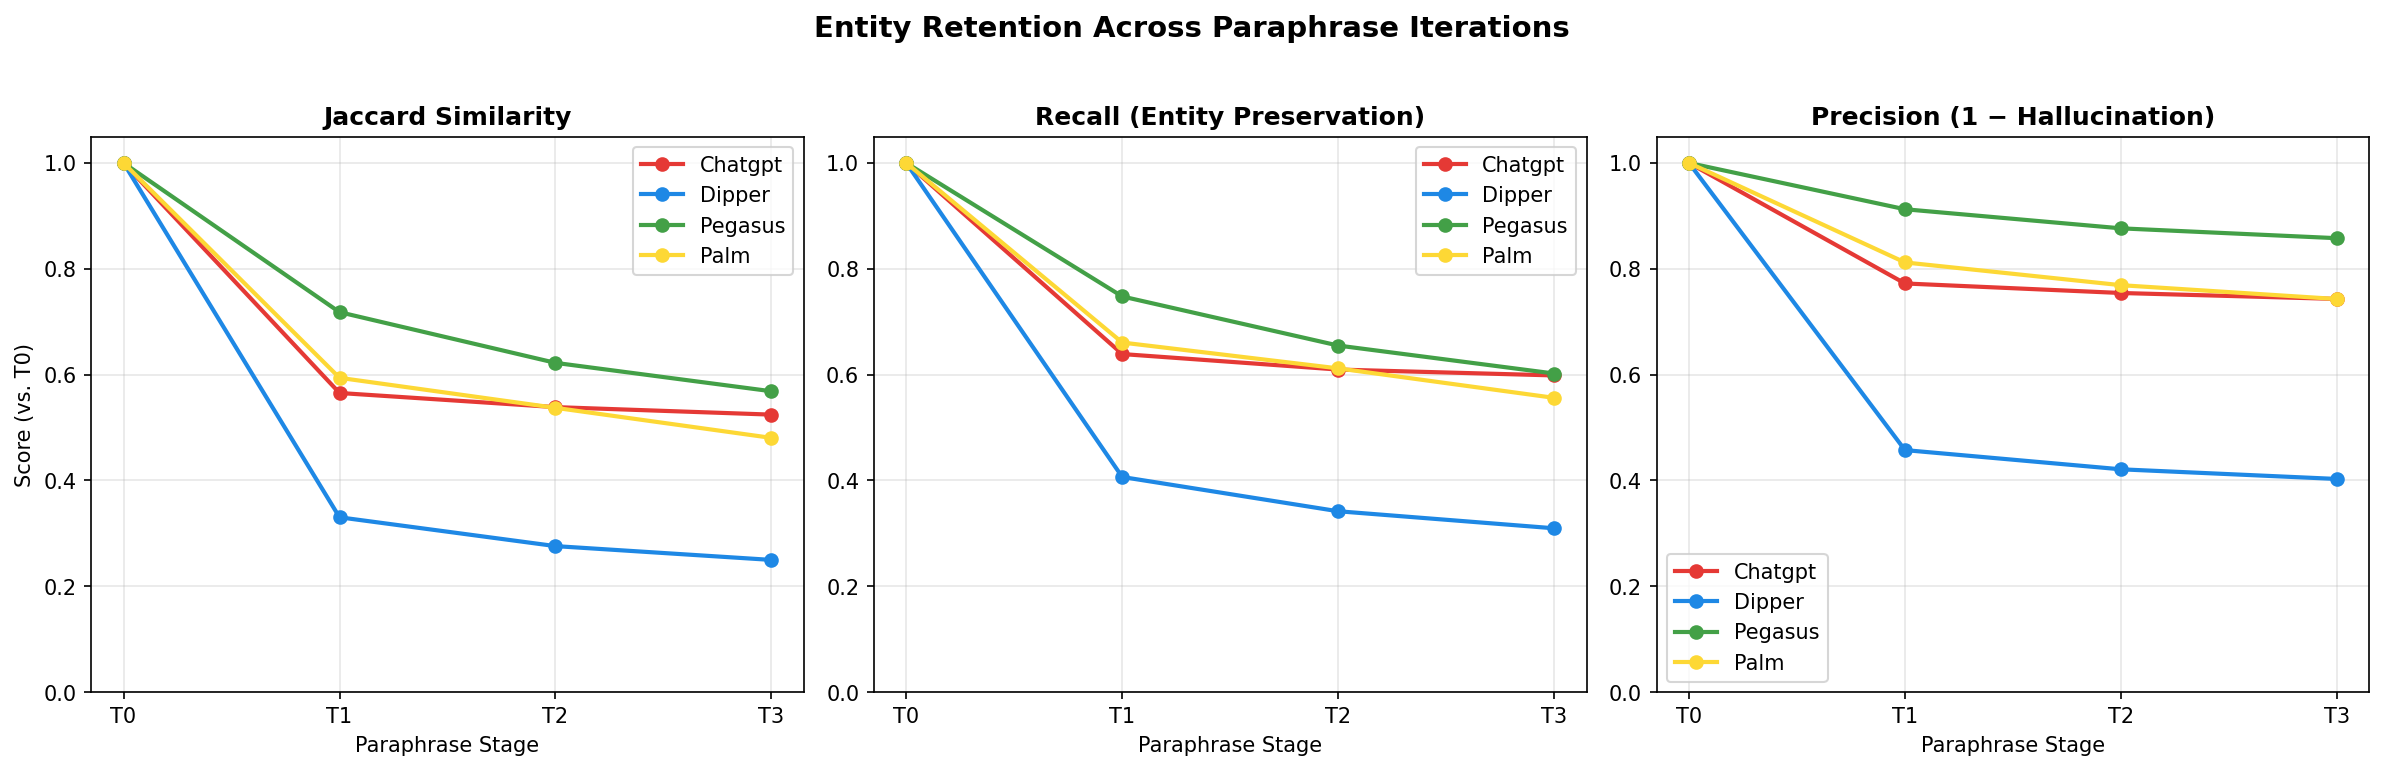
\includegraphics[width=\linewidth]{fig5_ner_decay_by_family.png}
  \caption{Entity retention (Jaccard, recall, precision) across iterations
  by paraphraser family. Dipper shows the steepest entity erosion; Pegasus
  preserves entities most faithfully.}
\end{figure}

\textbf{Paraphraser families differ dramatically in entity preservation.}
Dipper is the worst entity eraser, retaining only 31\% of original entities
at T3 (recall) with a precision of 0.40, indicating both aggressive dropping
\emph{and} frequent hallucination of new entities. Pegasus preserves 60\%
of entities with 86\% precision, consistent with its extractive design.
ChatGPT and PaLM fall between these extremes (recall 0.60 and 0.56 respectively).

\textbf{Paraphraser intensity scales entity loss proportionally.}
Pegasus(slight) retains 75\% of entities at T3 while Pegasus(full) retains
only 46\%---a 29pp gap. Dipper(low) preserves 65\% versus Dipper(high) at
just 5\%, demonstrating that increasing paraphraser aggressiveness
disproportionately destroys factual content.

\textbf{Domain vulnerability mirrors attribution patterns.} Scientific
text (sci\_gen) and news summaries (xsum) suffer the most entity loss,
likely because their specialized terminology and proper nouns are
unfamiliar to general-purpose paraphrasers. Colloquial domains (yelp, cmv)
retain entities better, paralleling the attribution results where
these domains also showed higher classification accuracy.

\subsection{Source Origin and Style Drift}

We investigate whether the \emph{origin} of the T0 text---human-authored
versus AI-generated---affects how much style is altered during paraphrasing.
POS cosine similarity between T0 and T1 was computed across all 7 datasets
grouped by source type.

Human-authored T0 texts show a mean POS cosine similarity of 0.964 after
paraphrasing, while AI-authored T0 texts show 0.961. This difference of
0.003 is negligible, indicating that \textbf{style drift is driven by the
paraphraser, not the source}. Whether the original text was written by a
human or an LLM, paraphrasers alter grammatical structure to a nearly
identical degree. This finding suggests that the ``fingerprint'' left by
paraphrasing is a property of the paraphraser itself rather than an
interaction between source and paraphraser.

\subsection{Multi-Modal Decay Audit}

We consolidate all analyses into a unified decay comparison across four
linguistic layers, measured at T3:

\begin{center}
\small
\begin{tabular}{llr}
\toprule
\textbf{Layer} & \textbf{Metric} & \textbf{T3 Score} \\
\midrule
Structure (skeleton) & POS Cosine Similarity & 0.870 \\
Semantics (hull)     & BERTScore F1          & 0.810 \\
Content (cargo)      & NER Jaccard           & 0.410 \\
Lexical (skin)       & BLEU-2                & 0.280 \\
\bottomrule
\end{tabular}
\captionof{table}{Multi-modal decay hierarchy at T3. The syntactic skeleton
is nearly unchanged; the lexical surface is almost entirely replaced.}
\label{tab:multimodal}
\end{center}

\begin{figure}[h]
  \centering
  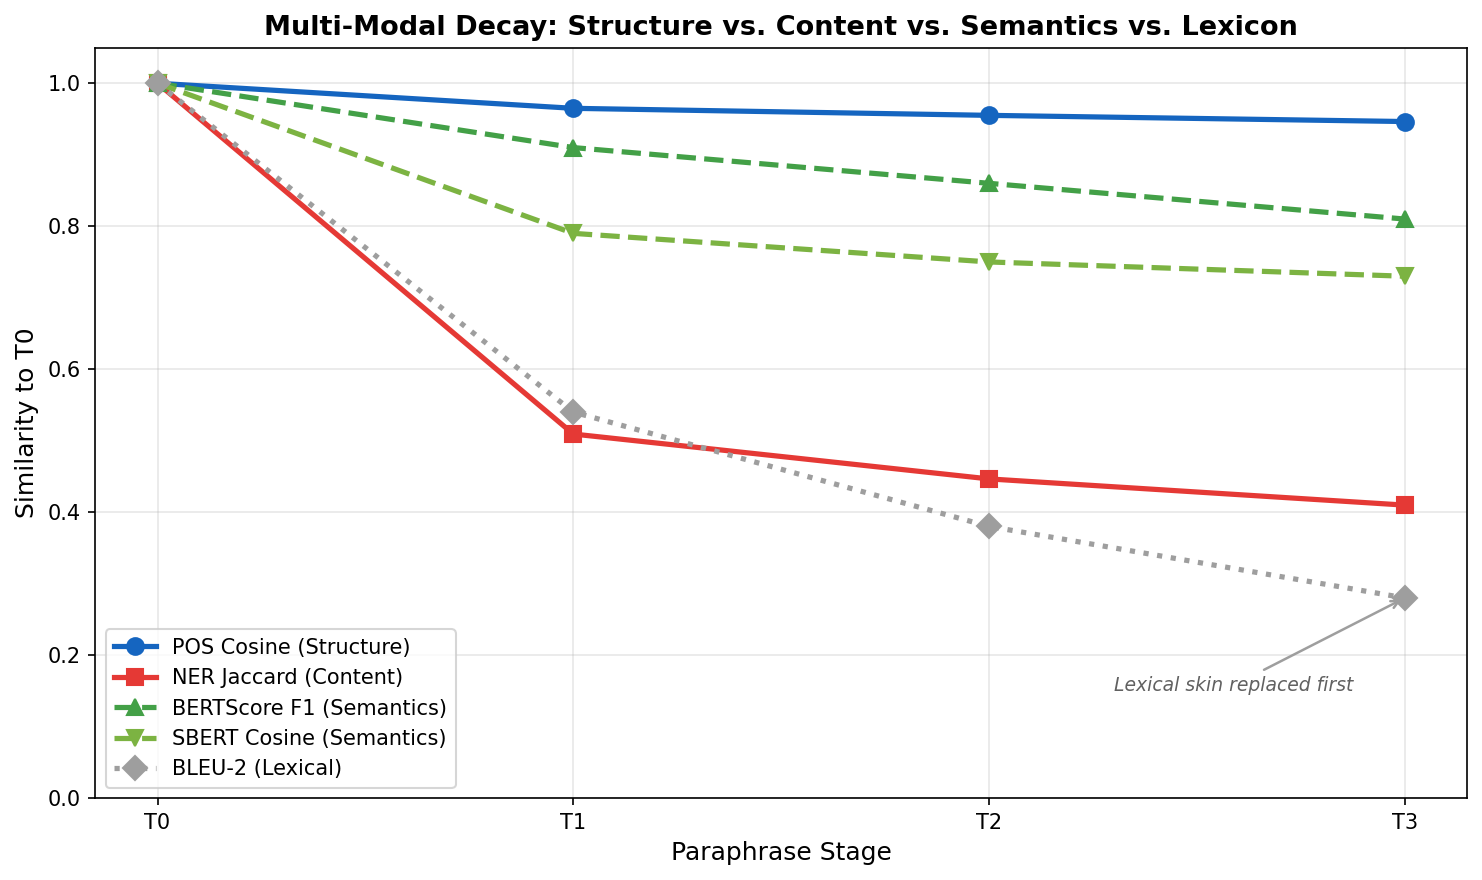
\includegraphics[width=\linewidth]{fig7_multimodal_audit.png}
  \caption{Multi-modal decay across T0--T3. Structure remains stable,
  semantics degrades slowly, content (entities) erodes significantly,
  and lexical surface is replaced rapidly.}
\end{figure}

\noindent The decay hierarchy is clear and consistent across all datasets:
$$\text{Lexical} > \text{Content} > \text{Semantics} > \text{Structure}$$

\noindent This ordering reveals that LLM paraphrasers operate in a specific
manner: they aggressively replace surface-level vocabulary (BLEU drops 72\%),
significantly alter factual referents (NER drops 59\%), moderately shift
distributional semantics (BERTScore drops 19\%), and barely touch
grammatical structure (POS cosine drops 13\%).

\section{Discussion}

\subsection{The Paradox of Authorial Identity}

Our multi-modal audit reveals a fundamental paradox: LLM paraphrasers
\emph{preserve meaning while erasing identity}. At T3, BERTScore remains
at 0.81 (meaning largely intact) while BLEU-2 drops to 0.28 (words almost
entirely replaced) and NER Jaccard falls to 0.41 (half of named entities
lost). The ship retains its shape and purpose, but the planks, cargo,
and paint have been systematically replaced.

This paradox has direct implications for academic integrity. A student
who runs a human-authored paper through three rounds of ChatGPT paraphrasing
produces text that conveys the same ideas, uses the same grammatical
structures, but shares fewer than 30\% of the original words and has lost
nearly half its named entities. Traditional plagiarism detectors that rely
on lexical overlap would fail to detect this transformation, yet the
intellectual content remains derivative.

\subsection{Answering the Research Questions}

\textbf{RQ1 (Style vs.\ Content Decay):} The decay hierarchy is
unambiguous: lexical features are replaced first (BLEU: $-$72\%), followed
by concrete content (NER: $-$59\%), then distributional semantics
(BERTScore: $-$19\%), and finally syntactic structure (POS: $-$13\%).
Style is eroded before content, and content before meaning. The ``planks''
of vocabulary are replaced long before the ``hull'' of meaning is
compromised.

\textbf{RQ2 (Point of No Return):} The point of no return has
\emph{not} been reached within three iterations. Attribution accuracy
remains at 79.5\% at T3, well above the 50\% chance baseline.
However, the sharpest erosion occurs at T1 ($-$14pp), with diminishing
returns at T2 and T3. This suggests a logarithmic decay curve where
the first paraphrase causes the most identity damage, with each
subsequent iteration producing smaller marginal effects.

\textbf{RQ3 (Paraphraser Fingerprints):} All four paraphraser families
leave identifiable fingerprints (overall F1 = 0.55, vs.\ 0.25 chance).
ChatGPT is the most identifiable (F1 = 0.70) due to its distinctive
treatment of punctuation and sentence structure. Crucially, we find
that style drift is driven by the paraphraser, not the source: human-authored
and AI-authored T0 texts show nearly identical POS drift after paraphrasing
(cosine 0.964 vs.\ 0.961), confirming that the fingerprint is a property
of the paraphraser itself.

\subsection{Implications}

\textbf{For academic integrity:} The combination of high semantic
preservation and low lexical overlap makes iterative paraphrasing a potent
tool for AI text laundering. However, our results suggest that
stylometric and entity-level features provide detection signals that
persist even when surface text is unrecognizable.

\textbf{For accessibility:} Dependency depth decreases monotonically
across all datasets ($-$3.9\% mean, $-$8.2\% max by T3), confirming
that paraphrasers systematically simplify syntax. While this may aid
comprehension, it comes at the cost of authorial voice and syntactic
diversity.

\textbf{For AI detection:} Entity retention analysis reveals that
paraphrasers not only drop original entities but also hallucinate
new ones (precision $<$ 1.0 at all stages). This entity hallucination
could serve as an additional signal for detecting AI-paraphrased text,
complementing existing stylometric approaches.

\section{Interactive Dashboard}

To enable exploration of these findings, we developed a Streamlit-based
``Style-Drift Dashboard'' that provides: (1) a document explorer for
side-by-side comparison of T0 and T3 texts with similarity scores; (2)
interactive decay curves with filterable paraphraser families and datasets;
(3) t-SNE identity trajectory visualizations with toggleable stages and
families; and (4) a multi-modal audit view consolidating all analysis
layers. The dashboard loads pre-computed experiment results and supports
real-time filtering for presentation and exploration.

\section{Limitations}

\textbf{Stylometric scope.} Stylometric features were extracted from
3 of 7 datasets (wp, xsum, yelp) due to computational cost. NER analysis
covers all 7 datasets but uses 500 samples per dataset rather than the
full corpus.

\textbf{Simple classifiers.} Attribution (Logistic Regression) and
fingerprinting (Random Forest) use traditional ML models. Fine-tuned
transformers would likely achieve higher accuracy, making our results
a lower bound on detectability.

\textbf{NER model limitations.} Entity extraction uses spaCy's
\texttt{en\_core\_web\_sm}, a relatively small model. A larger NER model
or domain-specific models (e.g., for scientific text) could yield more
accurate entity detection, potentially revealing different retention
patterns.

\textbf{Corpus scope.} All data comes from a single corpus
\cite{tripto2024} with four paraphraser families. Results may not
generalize to newer LLMs (GPT-4, Claude, Llama) or to longer documents.

\section{Conclusion}

We have presented a comprehensive multi-modal analysis of how iterative
LLM paraphrasing erodes linguistic identity across the Ship of Theseus
corpus. Our key contributions are:

\begin{enumerate}[leftmargin=*,topsep=2pt,itemsep=1pt]
  \item \textbf{A four-layer decay hierarchy:} lexical surface is
    replaced first (BLEU: 0.28 at T3), followed by named entities
    (Jaccard: 0.41), distributional semantics (BERTScore: 0.81), and
    syntactic structure (POS cosine: 0.87).
  \item \textbf{The point of no return is not reached by T3:}
    authorship attribution remains at 79.5\% accuracy after three
    iterations, with the sharpest drop at T1.
  \item \textbf{All paraphrasers leave identifiable fingerprints:}
    detectable above chance (F1 = 0.55), with ChatGPT most identifiable
    and style drift determined by the paraphraser, not the source text.
  \item \textbf{Entity hallucination as a new detection signal:}
    paraphrasers both drop original entities and fabricate new ones,
    providing a content-level complement to stylometric detection.
  \item \textbf{An interactive dashboard} for exploring style drift
    across documents, metrics, and paraphraser families.
\end{enumerate}

\noindent Returning to our central question: if every linguistic marker
is replaced by an AI but meaning remains, who is the author? Our data
suggests that three iterations of paraphrasing are insufficient to fully
erase authorial identity---the syntactic skeleton and residual stylometric
signatures persist. The ship has had most of its planks replaced and
much of its cargo lost, but its hull remains recognizably the same vessel.
The paradox of authorial identity, in our empirical framing, resolves
not as a binary but as a gradient: identity fades but does not vanish
within the paraphrase chains we studied.

\begin{thebibliography}{5}

\small

\bibitem{asthana2024} S. Asthana et al., ``Evauluating LLMs for Targested Concept Simplification for Domain-Specific Texts'' \textit{EMNLP}, 2024.
\bibitem{dong2017} L. Dong et al., ``Learning to Paraphrase for Question Answering,'' \textit{EMNLP}, 2017.
\bibitem{feng2010} L. Feng et al., ``A Comparison of Features for Automatic Readability Assessment,'' \textit{COLING}, 2019.
\bibitem{xu2015} W. Xu et al., ``Problems in Current Text Simplification Research:
New Data Can Help,'' \textit{TACL}, 2015.
\bibitem{zheng2018} J. Zheng et al., ``How do you correct run-on sentences it's not as easy as it seems,'' \textit{EMNLP}, 2018.
\bibitem{tripto2024} N. Tripto et al., ``A ship of theseus: Curious cases of paraphrasing in LLM-generated texts,'' \textit{ACL}, 2024.

\end{thebibliography}
\end{document}
